%%%%%%%%%%%%%%%%%%%%% Chapter 8 %%%%%%%%%%%%%%%%%%%%%%%%%%%%%%%%%
% Secure Aggregation: Cryptography & MPC
%%%%%%%%%%%%%%%%%%%%%%%%%%%%%%%%%%%%%%%%%%%%%%%%%%%%%%%%%%%%%%%%%
\motto{Secure Aggregation allows a server to compute the average of client updates without ever seeing any single update in the clear.}

\chapter{Secure Aggregation: Cryptography \& MPC}
\label{chap:secure_aggregation}

\abstract{Building on the decentralized architecture of Federated Learning, this chapter introduces the cryptographic protocols necessary to protect model updates from a curious or compromised central server. We explore the principles of Multi-Party Computation (MPC) and Secure Aggregation, using the analogy of "sealed envelopes" to explain pairwise masking. We analyze popular schemes like Bonawitz SecAgg \cite{bonawitz2017} and Homomorphic Encryption (CKKS), while addressing the critical trade-offs between cryptographic strength and system performance.}

\section{The Curious Server Problem}
\label{sec:curious_server}

In standard Federated Learning, clients send their model updates (gradients) to a central aggregator. While the raw data stays on the device, the gradients themselves can leak sensitive information. A "curious" server---one that follows the protocol but attempts to learn as much as possible---can use gradient inversion to reconstruct input data. Secure Aggregation is the cryptographic guardrail that prevents this by ensuring the server only ever sees the \textit{aggregate} sum, never the individual contributions.

\begin{svgraybox}
\textbf{The Analogy: Sealed Envelopes.} Imagine 100 hospitals want to sum their patient counts without revealing individual counts to a coordinator. Each hospital adds a unique random mathematical "mask" to their count before placing it in a sealed envelope. When the coordinator sums all the envelopes, the masks cancel each other out perfectly, revealing only the total sum.
\end{svgraybox}

\section{The Math of Pairwise Masking}
\label{sec:masking_math}

The goal of Secure Aggregation is to compute $\sum w_i$ without revealing any $w_i$. This is achieved through pairwise masking. 

Each client $i$ generates a random seed $s_{i,j}$ shared with client $j$. The client then uploads a masked update $u_i = w_i + r_i$, where $r_i$ is the sum of shared secrets:
\begin{equation}
r_i = \sum_{j \in N_i} (s_{i,j} - s_{j,i}) \pmod P
\end{equation}

\begin{figure}[t]
\centering
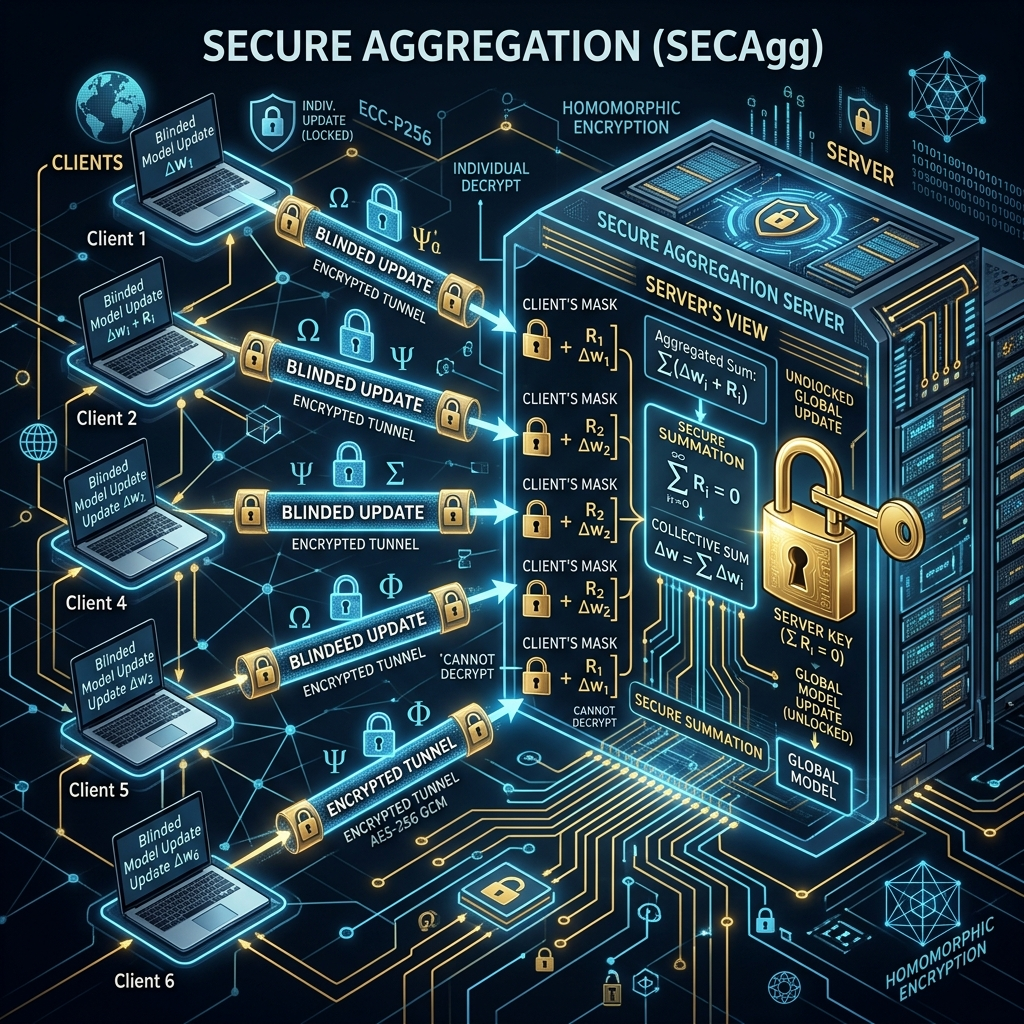
\includegraphics[width=\textwidth]{figures/ch8_secagg.png}
\caption{Secure Aggregation Logic: Pairwise masking ensures that individual updates are blinded during transit, while the masks cancel out at the server to reveal the aggregate sum.}
\label{fig:ch8_secagg}
\end{figure}

When the server aggregates all $u_i$, every secret $s_{i,j}$ is added exactly once and subtracted exactly once across the entire network, causing the masks to effectively vanish: $\sum u_i = \sum w_i$.

\section{Popular Schemes and Protocols}
\label{sec:secagg_protocols}

Choosing the right protocol depends on the computational constraints of the clients and the required robustness to network dropout.

\begin{table}
\caption{Comparison of Secure Computation Schemes}
\label{tab:secagg_schemes}
\begin{tabular}{p{3cm}p{3cm}p{4.5cm}}
\hline\noalign{\smallskip}
Scheme & Category & Best For \\
\noalign{\smallskip}\svhline\noalign{\smallskip}
Bonawitz SecAgg & MPC & Standard FL with high client dropout. \\
CKKS & Homomorphic Enc. & Deep Learning (Approximate arithmetic). \\
Paillier & Partial HE & Simple summation tasks. \\
\noalign{\smallskip}\hline\noalign{\smallskip}
\end{tabular}
\end{table}

\section{Trade-offs: Privacy vs. Performance}
\label{sec:secagg_tradeoffs}

Cryptographic defenses are not "free"; they introduce significant overhead that must be balanced by the Trustworthy AI Architect.

\begin{description}
  \item[Communication Overhead:] 
        Protocols like SecAgg require extra rounds for key exchange and secret sharing, which can increase latency in low-bandwidth environments.
  \item[Computational Cost:]
        Homomorphic Encryption (HE) can be 100x to 1000x slower than plaintext computation.
  \item[Robustness to Dropout:]
        If a client drops out after sending their masked update but before the unmasking phase, the server cannot recover the aggregate without specific "secret sharing recovery" mechanisms.
\end{description}

\section{Conclusion}
\label{sec:conclusion_secagg}

Secure Aggregation ensures that the central server remains a neutral aggregator rather than a potential spy. By combining the decentralization of FL with the cryptographic protection of MPC, we build the first layer of trust in distributed systems. However, cryptography only protects data \textit{in transit}. To protect the computation \textit{in use}, we must turn to the hardware layer, which we will explore in the next chapter on Trusted Execution Environments.


